\documentclass[11pt]{article}

\usepackage{a4wide}
\usepackage{graphicx}
\usepackage{epstopdf}
\usepackage{longtable}
\usepackage{caption}
\usepackage{pdflscape}
\usepackage{bbding}
\usepackage{pifont}
\usepackage{wasysym}
\usepackage{amssymb}
\usepackage[bookmarks]{hyperref}
\usepackage[utf8]{inputenc}

\title{AT3: Background Research}
\author{Rolf Jagerman, Laurens Versluis and Martijn de Vos}
\date{\today}

\begin{document}

\maketitle

\pagebreak

\section{Introduction (Martijn)}
Since the introduction of the internet in 1991 by CERN, we can't imagine a life without it. We make extensive use of applications like Facebook, Twitter and Netflix, applications that have only recently emerged. We're using the internet to share moments of our life, to run our business or for our entertainment by playing online games or watching videos. The innovation continues at a high rate and we're using the internet more and more.\\\\
We're not only connected with a desktop computer or laptop anymore: mobile devices are raising in popularity. Mobile devices like smartphones and tablets allows us to be always connected with each other. Popular mobile applications like WhatsApp and Instagram often have millions of users.\\\\
The increasing use of the internet also had its downsides. Cybercrime is a recent and growing problem: we're not always safe when we're browsing the worldwide web. Scamming and hacking are serious problems of the 21th century. In some countries like China and North Korea, the internet is censored and inhabitants are prohibited from visiting websites that are forbidden by the government. Anonymous communication could be a solution for these countries. A popular network for anonymous communication is Tor, however, as we will see Tor has many problems and does not scale very well. Another step in the right direction is Tribler, an anonymous peer-to-peer network created by the TU Delft. The rise of the internet also brings discussion about net neutrality, which is a highly debated issue in many countries.\\\\
In this research, we will first describe the Tor network in section II and look into its advantages and disadvantages. After that, the focus will move to Tribler and we will discuss the Tribler system in section III. We will delve into the various components Tribler contains of. In section IV, the focus will move to the mobile platform Android. We will look into the Android platform and discuss the advantages of the mobile operating system and what it could mean for Tor and Tribler. In section V, we will discuss a library that allows to run Python code on an Android device: Python for Android. One of the contributers to Python for Android is The Global Square. We will explain what The Global Square exactly is and what their goals are in section VI. Finally, we will discuss how we will be using the discussed software for our projects and we will elaborate what our project exactly is.

\pagebreak
\section{Tor (Rolf)}
	Tor, the second generation onion router, is a privacy-enhancing overlay network. Onion routing was first described by Chaum in his paper "Untraceable electronic mail, return addresses, and digital pseudonyms" \cite{chaum1981untraceable}. Tor is the most widely used and secure implementation of onion routing. It was first implemented in 1996 by the U.S. Navy Research Laboratory as a means to protect government and military communications from digital and physical attacks \cite{goldschlag1996hiding}.
	
	Tor uses the principle of onion routing to ensure secure communication between parties. Network traffic is encrypted and forwarded over a circuit of nodes. Each node in this circuit only knows the previous and next node. The communicating parties stay hidden when this circuit of independent nodes is sufficiently long.
	
	\begin{figure*}[!t]
		\centering
		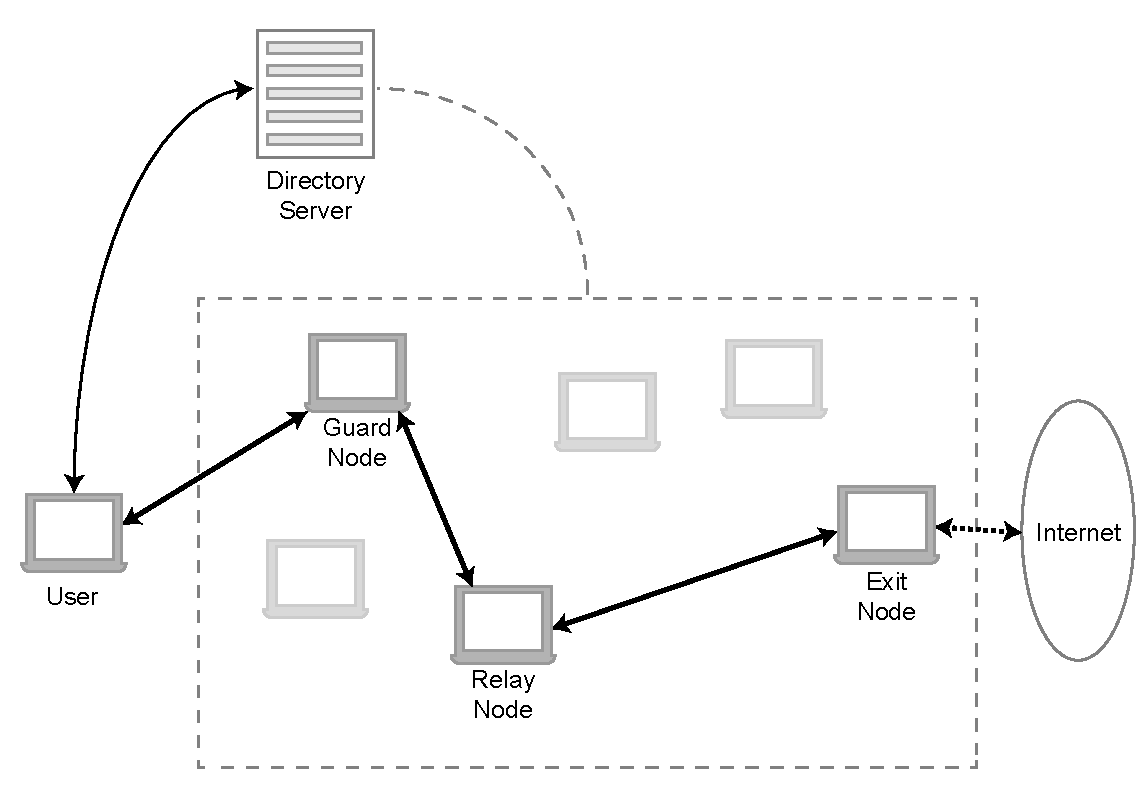
\includegraphics[width=0.8\textwidth]{graphics/tor.pdf}
		\caption{The components of the Tor network. After downloading the node list from the Directory Server, the user creates a circuit through a guard node, a relay node and an exit node. This circuit is used to communicate (anonymously) with the internet.}
		\label{fig:tor_layout}
	\end{figure*}
	
	There are several drawbacks to the current implementation of Tor. Centralized components, such as the directory server, act as a bottleneck and limit the number of possible users \cite{jagerman2014fifteen}. Since anonymity in a network such as Tor is directly linked to the number of active users this is an alarming situation.
	
	The Parallel and Distributed Systems group at Delft University of Technology has implemented a Tor-like protocol in the Python programming language. This protocol is currently used in a beta version of Tribler. In contrast to Tor, it does not use centralized components and is therefor a very scalable and secure way of communicating anonymously.

\section{Tribler}
In this section an overview of Tribler and its components is presented. We describe the new beta version that uses anonymous tunnels in depth. Furthermore we look at what specific dependencies Tribler relies on.

\subsection{What is Tribler? (Rolf)}
Tribler is a fully decentralized peer-to-peer file sharing platform developed by the Parallel and Distributed Systems group at Delft University of Technology. It has been in development for over 9 years and has a very mature and well-established code base. It allows users to search for and share files in a fully decentralized way. This decentralized nature of Tribler has several advantages over existing file sharing platforms. The lack of a centralized component makes it very scalable and practically impossible to bring down.

A new version of Tribler is currently in beta that includes a python implementation of a tor-like protocol. This enables users to share files anonymously and securely. By encrypting and routing traffic over a circuit of nodes, it ensures the communicating parties are oblivious of each other's virtual and physical location. More details about these anonymous tunnels can be found in section \ref{sec:anonymoustunnels}.

\subsection{M2Crypto (Martijn)}
Security is a big issue in the world of peer-to-peer networks. Not only do we want anonymous downloads, we also want confidentiality and integrity of our data. Confidentiality means that unauthorized parties can't see the exact content of the information. This could be achieved by encrypting the data. Integrity of the data means that the data is protected from being modified by other parties. Integrity can be achieved taking the hash of the data you receive and comparing it by taking the hash of the original message. If the hashes are not equal, the message has been modified. Confidentiality and integrity are important. When we're sending confidential data over the internet, it would not be beneficial if everyone has access to the message and can read what is being send. Integrity can play a role when transferring money to another bank account: we do not want an adversary to temper with the amount of money that is being transferred.\\\\
Some popular open source frameworks exists for these cryptographic tasks. A popular project is OpenSSL \cite{openssl}. OpenSSL implements the popular SSL and TLS protocols. These are cryptographic protocols that provides security when communicating over the internet. Besides that, OpenSSL provides libraries for various encryption and decryption protocols such as DES, RSA and RC4. OpenSSL also supports key exchange protocols such as Diffie-Hellman.\\\\
OpenSSL is written in C. To use the OpenSSL libraries in Python, one could use pyopenssl \cite{pyopensslgithub}, a interface for OpenSSL or M2Crypto \cite{m2cryptogithub} (M2Crypto stands for 'Me Too Crypto'), an OpenSSL wrapper. Tribler makes use of the M2Crypto library. The old homepage of the M2Crypto project \cite{m2crypto} explains what M2Crypto is:\\\\
\emph{M2Crypto is the most complete Python wrapper for OpenSSL featuring RSA, DSA, DH, HMACs, message digests, symmetric ciphers (including AES); SSL functionality to implement clients and servers; HTTPS extensions to Python's httplib, urllib, and xmlrpclib; unforgeable HMAC'ing AuthCookies for web session management; FTP/TLS client and server; S/MIME; ZServerSSL: A HTTPS server for Zope and ZSmime: An S/MIME messenger for Zope. M2Crypto can also be used to provide SSL for Twisted.}\\\\

\subsection{Dispersy}
Dispersy \cite{zeilemaker2013dispersy} is a fully decentralized system for data bundle synchronization used by Tribler. The system is designed in such a way that it is capable of running in a challenged network environment. Such an environment is often characterized by:
\begin{itemize}
\item Nodes randomly joining and leaving.
\item Delays in the network.
\item Nodes having different networking speeds (Edge, 3G, WiFi).
\item Nodes often being behind routers with Network Address Translating (NAT) firewalls.
\end{itemize}

All communication done by Dispersy uses UDP. Because up to 64\% of the internet is behind a NAT, they can use UDP firewall-NAT puncturing mechanisms.\\

In Dispersy, each node has a candidate list. A candidate list is a list of active connections within the node's overlay. A Dispersy node synchronizes in five steps:

\begin{enumerate}
\item First it selects a node from its candidate list.
\item It then selects a range of bundles to synchronize.
\item The node creates a Bloomfilter by hashing the selected bundles.
\item Then the node sends the created Bloomfilter to the selected node.
\item Finally, it pauses for a fixed interval to go back to step 1.
\end{enumerate}

The candidate list is divided into three sections: trusted nodes, nodes that have been successfully contacted in the past and nodes that have been connected in the past either trough an introduction-request or nodes that have been introduced.\\

A Bloomfilter uses a hash area consisting of \emph{N} bits, initially all set to zero. For each item that needs to be stored in the Bloomfilter, \emph{K} distinct addresses are generated using a hash of the item. The bits addressed in the Bloomfilter are then set to one. To check if an item is part of a Bloomfilter, one only has to generate the hash of that item and check if the addresses that are generated by the hash are one in the Bloomfilter.\\

After benchmarking Dispersy against Cassandra (the database system used by Facebook), they came to the conclusion that Dispersy performs better than Cassandra. By using Bloomfilters, Dispersy can scale to over 100,000 bundles to synchronize.

\subsection{Anonymous tunnels (Martijn)}
\label{sec:anonymoustunnels}
Recently, the research team of Tribler started to work on the implementation of anonymous downloads. Pull request 525 on the Tribler Github page \cite{pullrequest525} is an experimental build of Tribler with the implementation of anonymous communications. The anonymous communication is achived by using the Tor protocol. This protocol has been implemented in Python and uses a three-hop circuit for anonymous communication. Note that Tribler does not use the Tor network, only the Tor protocol. More information about Tor can be found in section II.\\\\
The anonymous tunnels are implemented in the Python module \emph{Tribler.community.anontunnel}. Taking the code as reference, we now describe various details of the anonymous tunnels.
\begin{itemize} 
\item The circuit setup is using the Diffie-Hellman key exchange protocol to establish a secure connection. The M2Crypto library is used for the Diffie-Hellman protocol.
\item The experimental code is using the Socks5 protocol for communication with other nodes. This code has been written by the Tribler team.
\item Dispersy is used as a cache system to keep track of the outstanding PING and EXTEND requests and of candidates used in CREATE and CREATED requests.
\item A circuit can be in four states: ready, extending, to be extended or broken.
\item There are nine different messages that can be send amongst nodes: create, created, extend, extended, data, ping, pong, puncture and stats.
\end{itemize}
In order to test the anonymous connections and the download speed, a special anonymous tab has been built into Tribler. Clicking on this tab brings up a graph of the current anonymous network as a graph. It also logs the circuit events such as the extend or creation of a circuit. When enough anonymous proxies are online, a 50MB test download file should start to download.\\\\

\begin{figure*}[!t]
		\centering
		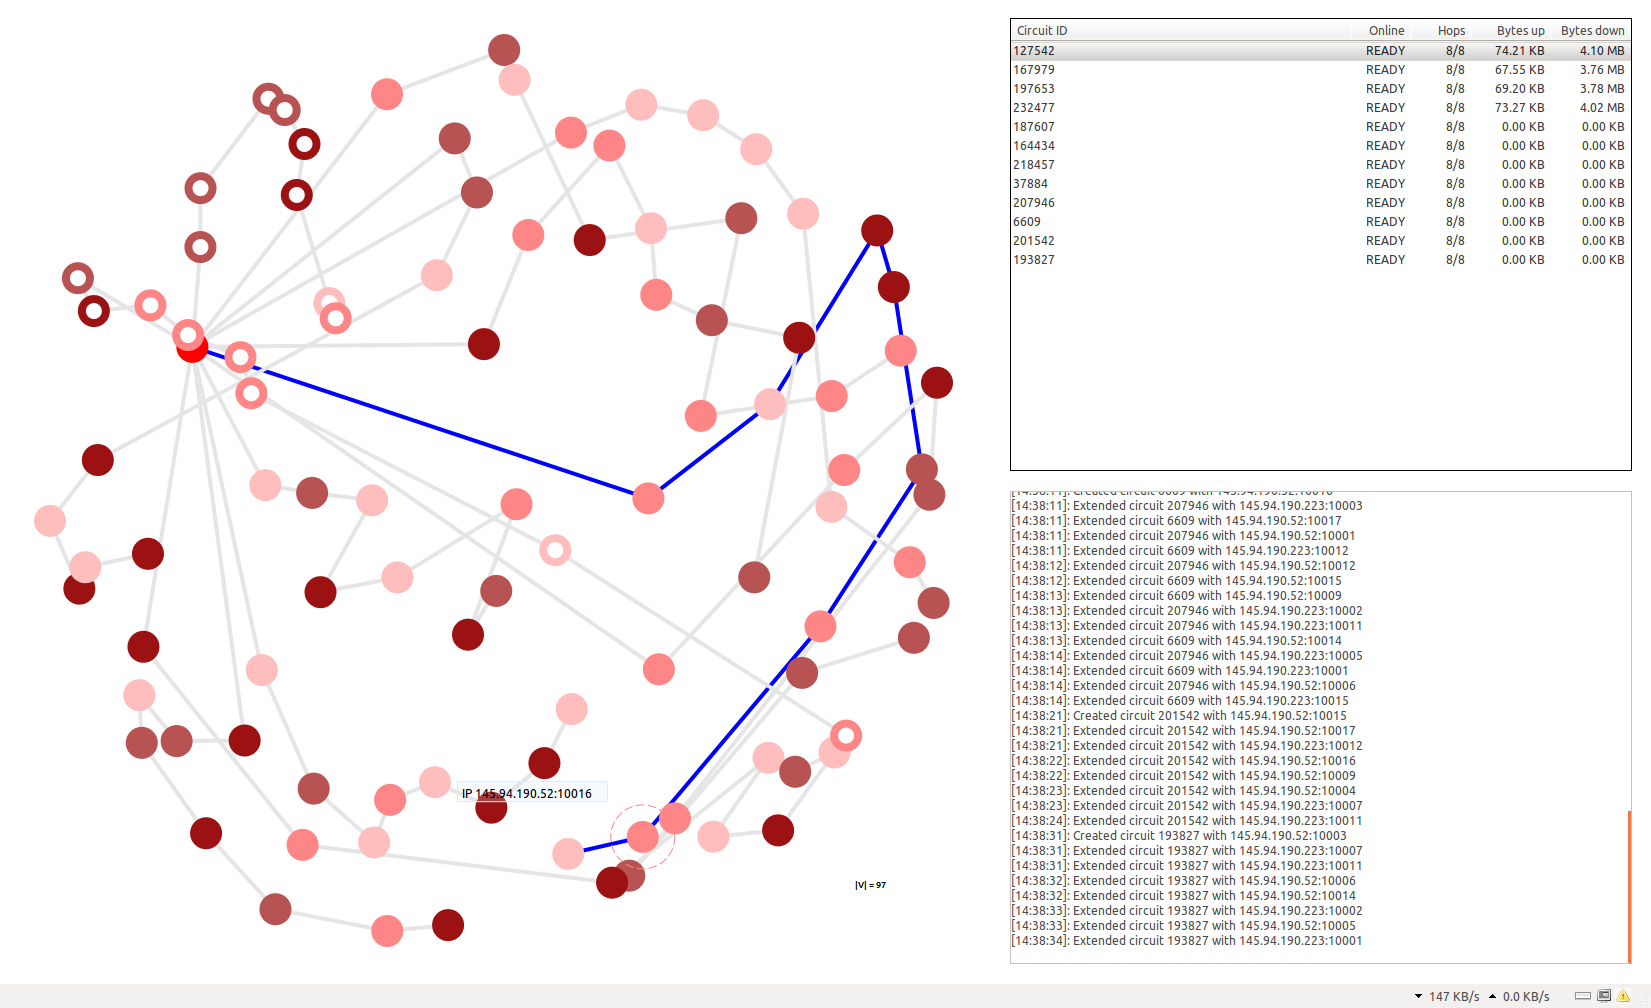
\includegraphics[width=0.8\textwidth]{graphics/8hop.png}
		\caption{The graphical user interface in Tribler that shows the anonymous network.}
		\label{fig:anon_downloads}
	\end{figure*}

\section{Motivation}
Worldwide the amount of mobile devices is growing fast. In 2013, there were 6.8 billion mobile subscriptions worldwide \cite{itustatistics}. This number is expected to exceed the world population in 2014 with 7.3 billion subscriptions. Android had a share of 81\% in Q3 of devices shipped \cite{forbesandroidmarket}.

This shows that there is a lot of potential gain on the Android market. Android is open source and can be modified more than a platform like iOs, on top of that is the Google Play not subject to a review before you can release your application, which allows for an easier deployment. Since a library called Python for Android already exists, it's also a more natural choice to develop it for Android since as stated earlier, the Tor-tunnel functionality is written in Python.

Besides the arguments stated above, a mobile application is an excellent way to attract more new users to Tribler. While the Tor project does have an Android app named Orbot, this app does not provide anonymous file transfer \cite{tororbot, googleplayorbot}. Orbot only serves as an anonymous proxy. On top of that, the structure of Tor is currently semi-centralized \cite{jagerman2014fifteen} where this app will be completely decentralized using Dispersy as synchronization system \cite{zeilemaker2013dispersy}. With the billions of mobile devices out there and no competition in this area, this app has a lot of potential to open a new way of anonymous file sharing while being on the go.

\section{Python for Android (Rolf)}
	The capability of running Python applications on Android devices is of paramount importance to the success of this project. Tribler is mostly written in the Python programming language and has dependencies on many Python libraries. Fortunately a tool called Python for Android allows us to build and bundle Python code and its dependencies into standalone Android APK packages.
	
	Python for Android uses Scripting Layer 4 Android (SL4A) to run Python in an Android environment. For performance reasons this layer uses the CPython binary compiled for the ARM architecture. This means that running python scripts will not work on other mobile architectures such as Intel Atom x86. This restriction however allows us to focus the development solely on the ARM architecture. This mitigates some of the difficulty of getting Tribler dependencies such as libtorrent to work cross-platform.
	
	Python for Android provides so called facades that interface python code with Android APIs. This makes it easy to utilize basic Android functionality directly from within Python.

\section{The Global Square (Martijn)}
Over the past years, Tribler had many contributors. One of these contributors is The Global Square (TGS). This organization has Github commits on the Dispersy and libswift project. They also worked on the Python for Android library and made steps to compile the libraries used by Tribler in Python for Android. In this section, we will first describe what TGS is and where they stand for. After that, we describe their contributions to Tribler.

\subsection{What is The Global Square?}
Roarmag, an online journal writing about the global struggle for real democracy, published a proposal in 2011 describing The Global Square: an online platform for our movement \cite{theglobalsquare}. Their proposal is to make an online platform where people of all nations can come together as equals to participate in the coordination of collective actions and the formulation of common goals and aspirations: The Global Square. This online platform could provide the following tools:
\begin{itemize}
\item An interactive map that lists all ongoing assemblies around the world.
\item A search option to find squares, events etc.
\item Individual pages for each local square/assembly where they can organize events and share information.
\item A public and private messaging system so individual users and groups can communicate with each other.
\end{itemize}
Traditional social media such as Facebook and Twitter, only allow to share and promote content. TGS encourage the active participation of citizens and the consolidation of working groups in a local and global context between individuals and assemblies. TGS should be multilingual and open source so everyone can be part of the platform.

\subsection{Their contribution to Tribler}
TGS has their own Github repository where they host contributions to various projects \cite{theglobalsquaregithub}. Notable are the contributions to the libswift and dispersy projects. The last commits to these projects are over a year ago.\\\\
Another important contribution has been done to the Python for Android project. TGS has added the libswift, netifaces and m2crypto libraries to the Python for Android project, making it possible to create an Android application bundle with these libraries included. This is an important contribution because it can be used as a first step to implement the Tribler community or anonymous tunnels on an Android device: Tribler is using some of these libraries.

\subsection{Our project (Martijn)}
We've discussed Tor, Tribler and have explained some libraries that Tribler is using and Python for Android. In this section, we will give an overview of our activities for the upcoming weeks.\\\\
The idea is to port the experimental code of pull request 525 to the Android device. This experimental code is written in Python so we have two options: either write the code of the anonymous tunnels in Java or use the Python for Android library to run the Python code on an Android device. We think the second options is the most easy. The Global Square already worked on porting some libraries to the Android so we can extend on their work. There are some other libraries we have to port such as libtorrent and Dispersy. Overall, this project will not be easy but if we succeed, it could be a big step towards anonymous streaming on the Android device.

\bibliographystyle{plain}
\bibliography{literature-research}

\end{document}
